\chapter{绪论}\label{DS01}

\par\medskip\noindent\textbf{知识导图}\par\smallskip
\begin{wideblock}\centering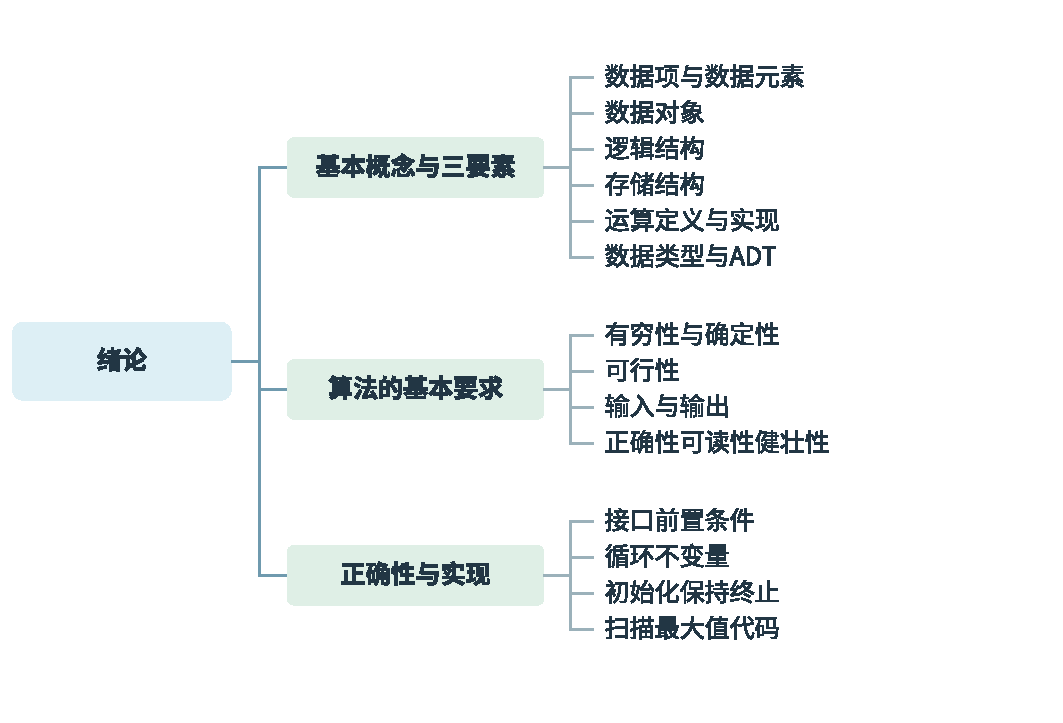
\includegraphics[width=\linewidth,height=168mm,keepaspectratio]{figures/map-01.pdf}\end{wideblock}\par\medskip\clearpage

\par\medskip\noindent\textbf{知识导图（续）}\par\smallskip
\begin{wideblock}\centering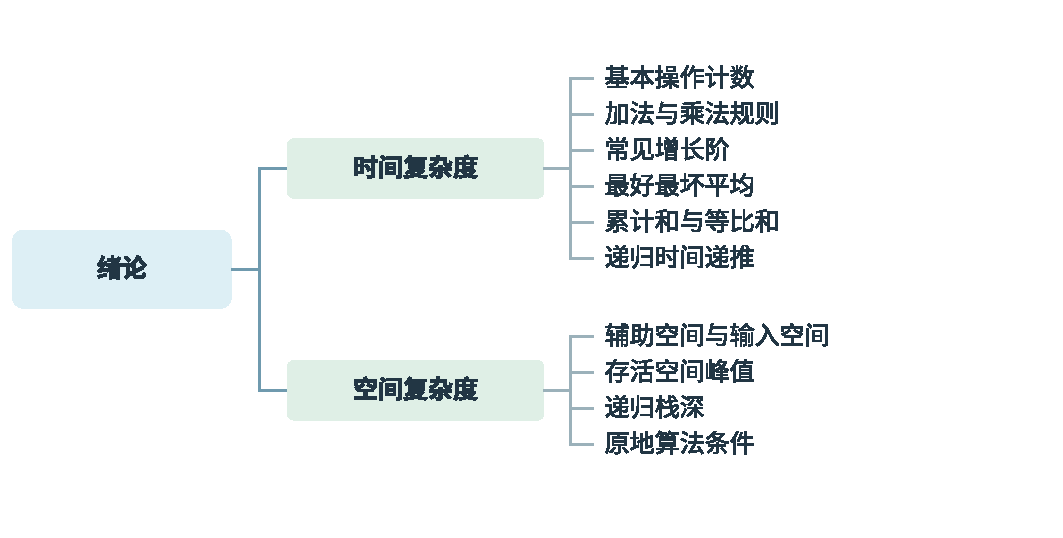
\includegraphics[width=\linewidth,height=168mm,keepaspectratio]{figures/map-02.pdf}\end{wideblock}\par\medskip\clearpage

本书中，\(n\) 表示输入规模。数组默认从 0 开始编号；线性表的``第 \(i\) 个元素''默认采用从 1 开始的位序，二者同时出现时会写明对应关系。指针变量保存结点地址，\texttt{p->\allowbreak{}next} 是 \texttt{p} 所指结点的后继指针域；\texttt{p=\allowbreak{}NULL} 表示 \texttt{p} 当前不指向任何有效结点。伪代码中的赋值号 \texttt{=\allowbreak{}} 不表示数学等式，循环边界和执行顺序同样是算法的一部分。

\section{逻辑关系怎样落实到存储}\label{DS01-01}

\textbf{数据元素}是数据的基本单位，一个元素可由若干数据项组成。例如一条学生记录是一个元素，学号和姓名是它的数据项。\textbf{数据对象}是性质相同的数据元素的集合。讨论数据结构时，还必须说明元素之间的关系：是排成先后序列，形成父子层次，还是由任意边相连。

\textbf{逻辑结构}描述元素之间的逻辑关系，不涉及具体地址。集合结构没有规定元素间的先后关系；线性结构中，除首尾元素外，每个元素都有一个直接前驱和一个直接后继；树形结构表达层次；图结构表达更一般的关联。栈和队列都以线性关系为基础，但允许的操作位置不同，因此属于不同的抽象数据类型。

\textbf{存储结构}是逻辑结构在计算机中的表示。顺序存储用相邻位置体现关系，链式存储用指针联系结点，索引存储另建索引以定位元素，散列存储由关键字计算位置。四者都只是表示方法，不能把``线性结构''直接等同于``连续地址''。线性表既能顺序存储，也能链式存储。

\subsection{例 1-1　值以外还要存什么}\label{DS01-ex1}

\begin{example}[配套例题]

〖1.1-005〗 在存储数据时，通常不仅要存储各数据元素的值，还要存储（　）。

A. 数据的操作方法　B. 数据元素的类型　C. 数据元素之间的关系　D. 数据的存取方法

\end{example}

\textbf{解析。} 若只保存若干值，就无法区分这些值原本属于一个序列、一棵树还是一张图。存储结构必须表达元素间的关系，答案为 \textbf{C}。关系未必另占一个专门字段：数组的相邻位置已隐含先后，链表则用指针显式记录后继。

运算的定义与实现也要分开。线性表的``按位序取值''是一种抽象运算；在数组上用下标访问、在链表上顺指针查找，则是两种实现。选择存储结构时，要同时考虑需要保存的关系和需要执行的运算，不能只看对象包含多少个元素。

\textbf{抽象数据类型（ADT）}把数据对象、关系和允许的操作合在一起描述，而不限定具体的机器实现。例如，栈规定 \texttt{push}、\texttt{pop} 及后进先出语义；顺序栈和链栈都能实现这一约定。

\section{算法怎样保证结束并得到正确结果}\label{DS01-02}

算法是求解一类问题的有限操作序列，通常要求有穷性、确定性、可行性、输入和输出：对合法输入，执行有限步后结束；每一步含义明确，并能在有限时间内完成；可以有零个或多个输入，至少有一个输出。输出不限于屏幕打印，也可以是返回值或修改后的数据状态。

算法的有穷性针对\textbf{每一次合法输入}。运行时间很长，仍可能满足有穷性；没有终止条件的服务程序可以是有用的程序，却不属于这里所说的有限求解算法。可行性要求操作能够执行，并不要求它在现实规模下足够快。正确、可读、健壮以及时空效率是进一步评价设计的维度；``必须具备的特性''与``希望达到的设计质量''属于不同层面的问题。

证明循环正确性，可以找一个每轮前后都保持的关系，称为\textbf{循环不变式}。例如，依次扫描数组求最大值：处理前 \(i\) 个元素后，\texttt{max} 等于这 \(i\) 个元素的最大值。证明分三步：初始化时说明该关系为何成立；每轮用下一个元素更新后说明它仍成立；终止时 \(i=n\)，由不变式可知结果覆盖了全体元素。此外还要说明循环变量不断接近边界，以排除关系成立却永不终止的程序。

空表、单元素、重复元素和查找失败都不是额外装饰。若把初始化写成 \texttt{max=\allowbreak{}A[0]}，输入规模就必须满足 \(n\ge1\)；若允许空数组，应另行约定失败时的返回值，不能继续访问 \texttt{A[0]}。

\section{怎样由执行次数得到时间复杂度}\label{DS01-03}

实际运行时间受机器、编译器和输入分布影响。比较算法的增长规律时，先选择一种基本操作，统计它的执行次数 \(T(n)\)，再研究 \(n\) 增大时的数量级。本书采用单位成本模型：定长整数的比较、赋值及一次数组访问都视为常数时间。若整数位数随输入增长，或者需要访问外存，这个假设就要重新检查。

\(T(n)=O(f(n))\) 给出渐近上界；\(T(n)=\Omega(f(n))\) 给出渐近下界；上下界同阶时记为 \(\Theta(f(n))\)。选择题通常用 \(O\) 表示所要求的紧数量级。\(3n^2+7n+9=\Theta(n^2)\)：当规模足够大时，低次项和常数因子都不会改变增长阶。把 \(O(n)\) 写成 \(O(2n)\) 并没有更精确地给出渐近阶。

\subsection{先看循环变量如何变化}\label{DS01-detail1}

\texttt{i+\allowbreak{}+\allowbreak{}} 经过 \(n\) 次增长到 \(n\)；\texttt{i*\allowbreak{}=\allowbreak{}2} 则约经 \(\log_2n\) 次到达循环边界。分析嵌套循环时，不能只数层数。若内层范围依赖外层变量，应先写出每轮次数再求和。例如：

\begin{codeblock}[language={}]
for i = 1 to n:
    for j = 1 to i:
        执行一次基本操作
\end{codeblock}

总次数为 \(1+2+\cdots+n=n(n+1)/2\)，所以是 \(\Theta(n^2)\)。外层和内层各有一个变量，并不意味着次数总是 \(n\times n\)；本例只是恰好达到平方阶。

\subsection{例 1-2　循环由累计和决定何时停止}\label{DS01-ex2}

\begin{example}[配套例题]

【2017】 下列函数的时间复杂度是（　）。

\BlueLines{3,4}
\begin{codeblock}[language=C]
int func(int n) {
    int i=0, sum=0;
    while (sum<n) sum += ++i;
    return i;
}
\end{codeblock}

A. \(O(\log n)\)　B. \(O(n^{1/2})\)　C. \(O(n)\)　D. \(O(n\log n)\)

\end{example}

\textbf{解析。} 条件检查的是 \texttt{sum}，应先把它写成循环次数的函数。执行 \(k\) 轮后，\texttt{i=\allowbreak{}k}，\(\mathrm{sum}=1+2+\cdots+k=k(k+1)/2\)。终止时，\(k\) 是满足 \(k(k+1)/2\ge n\) 的最小非负整数，即

\[k=\left\lceil\frac{\sqrt{1+8n}-1}{2}\right\rceil.\]

每轮只做常数次操作，故 \(k=\Theta(\sqrt n)\)，答案为 \textbf{B}。\texttt{sum} 最终约为 \(n\)，不能据此推出执行了 \(n\) 轮------每轮的增量本身也在增长。分析按题目给定的整数模型进行；实际实现还应防止固定字长溢出。

\subsection{例 1-3　两层循环为什么仍是线性时间}\label{DS01-ex3}

\begin{example}[配套例题]

【2022】 下列程序段的时间复杂度是（　）。

\begin{codeblock}[language=C]
int sum=0;
for (int i=1; i<n; i*=2)
    for (int j=0; j<i; j++)
        sum++;
\end{codeblock}

A. \(O(\log n)\)　B. \(O(n)\)　C. \(O(n\log n)\)　D. \(O(n^2)\)

\end{example}

\textbf{解析。} 外层的取值为 \(1,2,4,\ldots,2^k\)，其中 \(2^k<n\le2^{k+1}\)。各轮内层次数正好为这些值，总计

\[1+2+4+\cdots+2^k=2^{k+1}-1.\]

该和小于 \(2n\)，而当 \(n>1\) 时又不小于 \(n\) 的某个常数倍，故为 \(\Theta(n)\)，答案为 \textbf{B}。若把每一轮都估成最后一轮的 \(O(n)\)，再乘以外层轮数，得到的只是不紧的 \(O(n\log n)\) 上界，忽略了前几轮内层规模很小这一事实。

\subsection{最好、最坏与平均情况在比较什么}\label{DS01-detail2}

线性查找长度为 \(n\) 的表：目标在首位时比较 1 次；在末位或不存在时，通常比较 \(n\) 次。这是相同规模下不同输入造成的差异。\textbf{最坏时间}取规模为 \(n\) 的合法输入中的最大执行次数；\textbf{最好时间}取最小；\textbf{平均时间}还须说明输入的概率分布。不能把``平均''直接理解为最好与最坏的算术平均。

若 \(n\) 个元素被查找的概率相同，并且保证查找成功，则顺序查找的平均比较次数为 \((n+1)/2\)。若还可能失败，就要把失败概率及其代价计入；第7章将按查找模型分别计算。

递归算法先写出递推关系。例如，若每次只递归求解规模为 \(n-1\) 的一个子问题，并做常数工作，则 \(T(n)=T(n-1)+\Theta(1)=\Theta(n)\)。若产生两个规模为 \(n/2\) 的子问题，并在本层做线性合并，则 \(T(n)=2T(n/2)+\Theta(n)\)：每层总工作为 \(\Theta(n)\)，约有 \(\log_2n\) 层，总时间为 \(\Theta(n\log n)\)。不能只看到规模减半就写成对数时间；每层有多少个子问题同样决定总量。

\section{辅助空间中为何要计入递归栈}\label{DS01-04}

\textbf{辅助空间复杂度}衡量算法运行时所需的额外空间随输入规模增长的情况，一般不计输入本身占用的空间；题目对输出区是否计入另有约定时，按题意处理。本书比较排序时把归并辅助数组计入额外空间，不重复计算原数组。

几个循环变量只占 \(\Theta(1)\) 空间，循环执行一万次也不需要同时保存一万个变量。相反，递归调用尚未返回时，调用记录必须同时保留参数、返回位置和局部状态。递归求和每层只用常数空间，但同一时刻最多存在 \(n\) 层调用，因此辅助空间为 \(\Theta(n)\)；时间与空间同阶只是这个例子的特点，并非所有递归都如此。

若一次调用先处理左半、返回后再处理右半，左右子树的递归调用就不会全程同时展开。二叉树遍历的调用总数为 \(\Theta(n)\)，最大栈深为树高 \(h\)，故递归辅助空间是 \(O(h)\)。完全二叉树中 \(h=\Theta(\log n)\)；单支链中 \(h=\Theta(n)\)。这里不能用``访问了 \(n\) 个结点''代替``同时保留了多少层状态''。

\textbf{原地算法}通常允许常数个辅助单元。只数递归代码中有几个显式变量而忽略调用栈，就可能误判为原地算法。快速排序即使在原数组上划分，递归栈仍要计入：普通实现平均 \(O(\log n)\)，最坏 \(O(n)\)；第8章会解释两者分别对应怎样的划分。

\section{由导图辨清对象、结构、类型与运算}\label{DS01-map}

\begin{definition}[数据结构的三要素]

一个数据结构要同时回答：对象中有哪些元素，元素之间是什么逻辑关系，需要提供哪些运算。存储结构负责把这些关系及操作落实为计算机中的表示与实现。数据项是构成元素的不可分割单位；记录由多个数据项构成，却仍可作为一个元素整体处理。

\end{definition}

数据类型由一个值的集合及定义在该集合上的操作组成。原子类型的值不再分解，结构类型的值可分解为成分；抽象数据类型进一步强调对使用者可见的对象、关系和操作语义，将实现细节藏在接口之后。逻辑结构与存储结构不是一一对应：同一逻辑结构可以有多种表示，同一种链式表示也能用于线性表、树、图。

\begin{wideblock}

\par\medskip\noindent\begin{minipage}{\linewidth}\fontsize{9.3}{12}\selectfont\begin{tabularx}{\linewidth}{@{}YYYY@{}}
\toprule\noalign{}
\begin{minipage}[b]{\linewidth}\raggedright
判断维度
\end{minipage} & \begin{minipage}[b]{\linewidth}\raggedright
需要说明什么
\end{minipage} & \begin{minipage}[b]{\linewidth}\raggedright
例子
\end{minipage} & \begin{minipage}[b]{\linewidth}\raggedright
不能直接推出什么
\end{minipage} \\
\midrule\noalign{}


逻辑结构 & 元素间关系 & 序列、层次、任意关联 & 是否使用连续地址 \\
存储结构 & 地址与链接的表示 & 顺序、链式、索引、散列 & ADT允许的操作一定相同 \\
运算定义 & 输入、输出与前后条件 & 取第i个元素、插入 & 具体执行多少次访问 \\
运算实现 & 在已定表示上怎样执行 & 数组寻址、逐结点扫描 & 另一种表示下代价也相同 \\
\bottomrule\end{tabularx}
\end{minipage}\par\medskip

\end{wideblock}

\section{用一个完整算法连接特性、正确性与代价}\label{DS01-code}

\begin{methodbox}[先写接口契约，再写循环]

以求数组最大值为例：合法输入为长度\(n\ge1\)的有效数组；返回值应等于数组中某个元素，且不小于任意元素。允许空输入时，必须把失败作为接口的一部分；不能凭空取一个数充当所有整数数组的最大值。

\end{methodbox}

\BlueLines{3,6,8}
\begin{codeblock}[language=C++]
#include <cstddef>
bool maximum(const int* a, std::size_t n, int& answer) {
    if (n == 0 || a == nullptr) return false;
    int best = a[0];
    for (std::size_t i = 1; i < n; ++i)
        if (a[i] > best) best = a[i];
    answer = best;
    return true;
}
\end{codeblock}

上面的C++17接口以布尔返回值区分``空数组没有最大值''和``最大值恰为0''，失败时不修改answer。若a非空，还要求它实际指向至少n个有效元素；仅检查指针非空并不能检验其可访问长度。后续指针操作同样必须满足有效结点前提。

\begin{proof}[扫描最大值的循环证明]

进入第\(i\)轮前，不变量为\texttt{best=\allowbreak{}max(\allowbreak{}a[0..i-1])\allowbreak{}}。初始化\(i=1\)时，唯一已处理元素为\(a[0]\)；比较\(a[i]\)后取较大者，不变量扩展到前\(i+1\)个元素。\(i\)严格递增且上界为\(n\)，故循环终止；终止时处理全部元素，返回正确最大值。非空输入恰有\(n-1\)次元素大小比较，所以时间为\(\Theta(n)\)，额外存储为\(\Theta(1)\)。

\end{proof}

\section{渐近分析的运算规则及适用条件}\label{DS01-rules}

\begin{theorem}[加法取主阶，嵌套先计实际次数]

若两段代码依次执行，时间为\(T_1(n)+T_2(n)\)，可按最大数量级归并；若一段工作被重复\(k(n)\)次且每次代价有统一紧界，才可直接相乘。内层范围随外层变化时，先写求和。常数底的对数只相差常数因子。

\end{theorem}

常见增长次序（\(c>1\)为固定常数）为

\[1\prec\log n\prec n\prec n\log n\prec n^2\prec n^3\prec c^n\prec n!.\]

\(O\)上界并不唯一：线性算法当然也属于\(O(n^2)\)，但题目通常要求最紧的常见阶。最好/最坏描述同规模输入的选择，\(O/\Omega/\Theta\)描述函数之间的界，不能将两组概念机械配对为``O只表示最坏''。

空间必须数\textbf{同一时刻仍存活的状态}。两段代码顺序使用并释放临时数组时，峰值可取各段最大值；两个数组同时保留时才相加。循环内每轮复用一个长度\(n\)的临时数组，即使循环\(n\)轮，峰值仍为\(\Theta(n)\)而非\(\Theta(n^2)\)。递归每层若分配不同规模的数组，必须沿一条同时活跃的调用链求和，而非只用层数乘最外层空间。

\section{历史错题指向的辨析}\label{DS01-errors}

算法必须具备五项基本特性；正确性、可读性、健壮性以及时空效率则是进一步评价设计的维度。CPU实际耗时受机器与实现影响，并非只由抽象算法决定；也允许以更多空间换取更少时间。配套单选对``衡量优劣''的概括存在措辞歧义，复习时应掌握这几个层次的区别，不把时空效率当作全部质量条件。做复杂度题则先找真正的停止量，列累计和或等比和，避免将变量最终值直接当作循环次数。

\section{主动回忆自测}\label{DS01-check}

第1题为配套题，其余为自拟补充。先遮住答案，说明停止条件、存活空间与表示关系。

\begin{recallcard}[合上正文，沿导图复述]

\begin{enumerate}
\def\labelenumi{\arabic{enumi}.}
\tightlist
\item
  【2019】设n是描述问题规模的非负整数，程序段 \texttt{x=\allowbreak{}0;\allowbreak{} while(\allowbreak{}n>\allowbreak{}=\allowbreak{}(\allowbreak{}x+\allowbreak{}1)\allowbreak{}*\allowbreak{}(\allowbreak{}x+\allowbreak{}1)\allowbreak{})\allowbreak{} x=\allowbreak{}x+\allowbreak{}1;\allowbreak{}} 的时间复杂度是（　）。A. \(O(\log n)\)　B. \(O(n^{1/2})\)　C. \(O(n)\)　D. \(O(n^2)\)
\item
  一段算法循环调用一个无递归函数 \(n\) 次，每次函数使用 10 个整数局部变量。仅考虑这些局部变量，辅助空间是 \(O(n)\) 还是 \(O(1)\)？
\item
  一个对象采用链式存储，能否据此断定它的逻辑结构是一棵树？
\item
  数据项、数据元素、数据对象之间是什么关系？ADT是否规定必须用数组实现？
\item
  算法的五项特性与正确性、健壮性有什么区别？``输入''必须从键盘读入吗？
\item
  单个循环变量连续翻倍，和外层翻倍但内层执行i次，两者为什么不是同一个阶？
\item
  顺序执行两段各需n个临时单元的代码，峰值空间一定是2n吗？
\item
  递归每次将规模减半、每层只用常数空间，时间是否一定是对数阶？还缺什么信息？
\end{enumerate}

\end{recallcard}

\subsection{核对答案}\label{DS01-recall-extra}

{\tcbset{SNbase/.append style={breakable=false}}\begin{recallcard}[先核条件，再核结论]

\begin{enumerate}
\def\labelenumi{\arabic{enumi}.}
\item
  \textbf{B}。次数恰为 \(\lfloor\sqrt n\rfloor\)：终止时 \(x^2\le n<(x+1)^2\)，仍为平方根数量级，但停止方程与例 1-2的累计和不同。2. \(O(1)\)：前一次调用返回后，局部空间可以复用。3. 不能。链式存储只是一种表示方法，线性表、树和图都可以采用。
\item
  元素是处理的基本单位，由数据项组成；对象是同性质元素的集合。ADT规定抽象语义而不限定表示。
\item
  五项特性描述作为有限求解算法的要求；正确性等描述设计质量。输入可由参数、已存数据等提供，并不限定交互方式。
\item
  前者轮数为对数；后者基本操作数为1+2+4+\ensuremath{\cdots}，是线性量级。
\item
  不一定。若前段的临时空间结束后可复用，峰值只需n个量级；若两段结果必须同时保留才相加。两者渐近阶均为Θ(n)，但实际峰值不同。
\item
  还要知道每层产生几个子问题、每个调用做多少非递归工作。两个半规模递归和一个半规模递归具有不同调用总量。
\end{enumerate}

\end{recallcard}}
